\documentclass[12pt]{standalone}
\usepackage{tikz}
\usetikzlibrary{arrows.meta}

\usepackage{anyfontsize} % allows arbitrary font sizes
\usepackage{lmodern} % better font scaling

\makeatletter
\renewcommand\normalsize{%
  \@setfontsize\normalsize{16pt}{19pt}%
}
\renewcommand\small{%
  \@setfontsize\small{12pt}{14pt}%
}
\renewcommand\Large{%
  \@setfontsize\Large{20pt}{24pt}%
}
\makeatother

\begin{document}

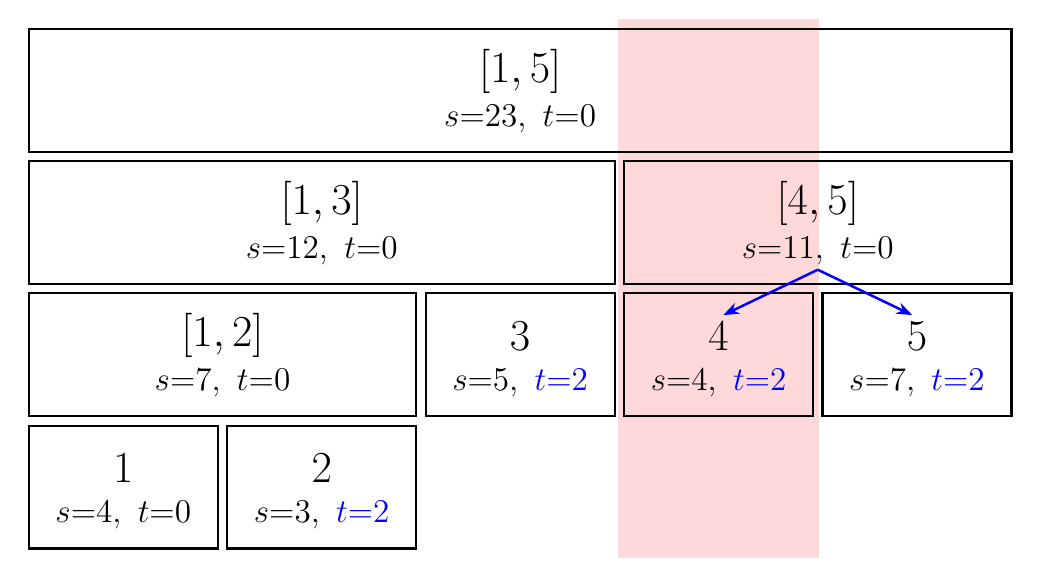
\begin{tikzpicture}[thick,scale=1.2]
% query(4): the tag of [4,5] is pushed down; leaf 4 holds the answer.
\draw[fill=red!15, draw=none, overlay] (6.24,0.1) rectangle (8.36,-5.6);
% Layer 1.
\draw (0.0,0.0) rectangle (10.4,-1.3);
\node at (5.2,-0.45) {$[1,5]$};
\node at (5.2,-0.95) {\small $s{=}23,\ t{=}0$};
% Layer 2.
\draw (0.0,-1.4) rectangle (6.2,-2.7);
\node at (3.1,-1.85) {$[1,3]$};
\node at (3.1,-2.35) {\small $s{=}12,\ t{=}0$};
\draw (6.3,-1.4) rectangle (10.4,-2.7);
\node at (8.35,-1.85) {$[4,5]$};
\node at (8.35,-2.35) {\small $s{=}11,\ t{=}0$};
% Layer 3.
\draw (0.0,-2.8) rectangle (4.1,-4.1);
\node at (2.05,-3.25) {$[1,2]$};
\node at (2.05,-3.75) {\small $s{=}7,\ t{=}0$};
\draw (4.2,-2.8) rectangle (6.2,-4.1);
\node at (5.2,-3.25) {$3$};
\node at (5.2,-3.75) {\small $s{=}5,\ {\color{blue}t{=}2}$};
\draw (6.3,-2.8) rectangle (8.3,-4.1);
\node at (7.3,-3.25) {$4$};
\node at (7.3,-3.75) {\small $s{=}4,\ {\color{blue}t{=}2}$};
\draw (8.4,-2.8) rectangle (10.4,-4.1);
\node at (9.4,-3.25) {$5$};
\node at (9.4,-3.75) {\small $s{=}7,\ {\color{blue}t{=}2}$};
% Layer 4.
\draw (0.0,-4.2) rectangle (2.0,-5.5);
\node at (1.0,-4.65) {$1$};
\node at (1.0,-5.15) {\small $s{=}4,\ t{=}0$};
\draw (2.1,-4.2) rectangle (4.1,-5.5);
\node at (3.1,-4.65) {$2$};
\node at (3.1,-5.15) {\small $s{=}3,\ {\color{blue}t{=}2}$};
% Push-down: the tag of [4,5] is handed to both children.
\draw[-{Stealth[length=2mm]}, blue, line width=.9pt] (8.35,-2.55) -- (7.35,-3.03);
\draw[-{Stealth[length=2mm]}, blue, line width=.9pt] (8.35,-2.55) -- (9.35,-3.03);
\end{tikzpicture}

\end{document}
